\documentclass[conference,a4paper]{IEEEtran}
\IEEEoverridecommandlockouts

% Packages
\usepackage{cite}
\usepackage{amsmath,amssymb,amsfonts}
\usepackage{algorithmic}
\usepackage{graphicx}
\usepackage{textcomp}
\usepackage{xcolor}
\usepackage{booktabs}
\usepackage{tabularx}
\usepackage{url}
\usepackage{microtype}

\def\BibTeX{{\rm B\kern-.05em{\sc i\kern-.025em b}\kern-.08em
    T\kern-.1667em\lower.7ex\hbox{E}\kern-.125emX}}

\begin{document}

\title{India's AI Infrastructure Sovereignty: A Five-Pillar Resilience Framework for Mitigating Strategic Dependencies}

\author{\IEEEauthorblockN{Adarsh Singh}
\IEEEauthorblockA{\textit{Department of Computer Science \& Engineering} \\
\textit{Amity School of Engineering and Technology, Amity University Madhya Pradesh}\\
Gwalior, India \\
pratiksingh79.in@gmail.com}
}

\maketitle

\begin{abstract}
As artificial intelligence transitions from an algorithmic curiosity to the core nervous system of modern national defense, scientific discovery, and economic productivity, access to scalable compute infrastructure has emerged as an indispensable sovereign capability. However, the contemporary global AI supply chain exhibits unprecedented geographic and corporate concentration: advanced photolithography tools, leading-edge semiconductor foundries, advanced packaging facilities, and AI accelerator architectures each exhibit Herfindahl-Hirschman Index (HHI) values exceeding 7,000, creating profound systemic chokepoints susceptible to weaponized interdependence. This paper investigates the strategic imperative of AI infrastructure sovereignty for India. We propose the India AI Infrastructure Resilience Framework (IAIRF), a unified five-pillar analytical model that deconstructs the national compute stack into: (1) Silicon Fabrication and Advanced Packaging, (2) High-Density Data Centres and Thermal Engineering, (3) Power Grid Integration and Clean Energy, (4) Sovereign Foundation Models and Multilingual Data Trusts, and (5) Strategic Governance and Multilateral Diplomacy. Applying empirical data from recent industrial policies—including the \textyen 1,27,500 crore Semicon India 2.0 outlay and the \textyen 10,372 crore IndiaAI Mission—we formulate a quantitative Vulnerability Index ($V_i$) and an inter-pillar Cascading Dependency Matrix ($\mathbf{D}$). Our analysis exposes the critical ``borrowed silicon'' paradox underpinning India's 45,000 shared GPU pool and models the unit economics of subsidized compute (\textyen 65/GPU-hour) versus foreign commercial clouds. Finally, we establish a sequenced three-horizon policy roadmap to transition India from passive hardware dependency to resilient, coordinated specialization.
\end{abstract}

\begin{IEEEkeywords}
Artificial Intelligence Infrastructure, Compute Sovereignty, Semiconductor Value Chain, Data Centres, Economic Statecraft.
\end{IEEEkeywords}

\section{Introduction}
Over the past decade, artificial intelligence (AI) has undergone a structural paradigm shift, evolving from distributed statistical software into an ultra-compute-intensive industrial apparatus. Training frontier multimodal foundation models now demands superclusters comprising tens of thousands of high-bandwidth accelerators operating continuously across multi-megawatt facilities \cite{geopoliticscompute2026}. Consequently, computing capacity—measured in ExaFLOPs of tensor operations—has become as fundamental to national sovereignty, state power, and industrial competitiveness as domestic energy grids, telecommunications backbones, and defense industrial capacity \cite{sastry2024governance, pau2025sovereignty}.

This infrastructural transformation coincides with an acute geopolitical restructuring characterized by ``weaponized interdependence'' \cite{farrell2019weaponized}, wherein global economic network hubs are leveraged by hegemon states for extraterritorial strategic coercion. The global hardware substrate sustaining generative AI is singularly vulnerable to such dynamics. From ASML's monopoly on extreme ultraviolet (EUV) photolithography to TSMC's concentration of sub-5nm wafer fabrication and NVIDIA's dominant accelerator ecosystem, critical nodes of the value chain exhibit extreme monopolistic concentration \cite{akimitsu2026supply, miller2022chipwar}.

For India, this reality poses a profound strategic paradox. While the nation boasts the world's third-largest AI ecosystem by vibrant developer activity, housing over 20\% of the global chip design workforce and producing recognized models such as Sarvam 30B/105B and the BharatGen consortium \cite{stanford_hai2025, meity2026semicon}, its foundational physical hardware remains almost entirely imported. The 45,000+ graphics processing units (GPUs) currently subsidized under the national IndiaAI Mission run on foreign-designed, Taiwanese-fabricated silicon subject to United States Export Administration Regulations (EAR) \cite{thakker2026sovereign, cetas2026semicon}. An export embargo, licensing restriction, or conflict in the Taiwan Strait would instantly halt compute replenishment across the Indian subcontinent.

Existing academic literature has addressed elements of this vulnerability in conceptual silos: semiconductor supply-chain analysts examine wafer fabs \cite{ezell2024india, nishant2026semicon}; energy researchers quantify data centre power loads \cite{iea2024energy, lbnl2025energy}; and policy scholars evaluate data governance \cite{pau2025sovereignty}. Crucially, no empirical study has yet integrated these disparate physical, electrical, and institutional domains into a single quantitative resilience framework calibrated for the Indian economy.

This paper addresses that gap through three primary contributions:
\begin{enumerate}
    \item We introduce the \textit{India AI Infrastructure Resilience Framework (IAIRF)}, decomposing national compute sovereignty into five interconnected pillars.
    \item We formulate a quantitative Vulnerability Index ($V_i$) and an empirical Cascading Dependency Matrix ($\mathbf{D}$) evaluating cross-pillar failure propagation and unit economic sustainability.
    \item We present a sequenced three-horizon strategic policy roadmap demonstrating how a rising middle power can attain resilient ``coordinated specialization'' without pursuing fiscally ruinous full-stack autarky.
\end{enumerate}

\begin{figure}[t]
\centering
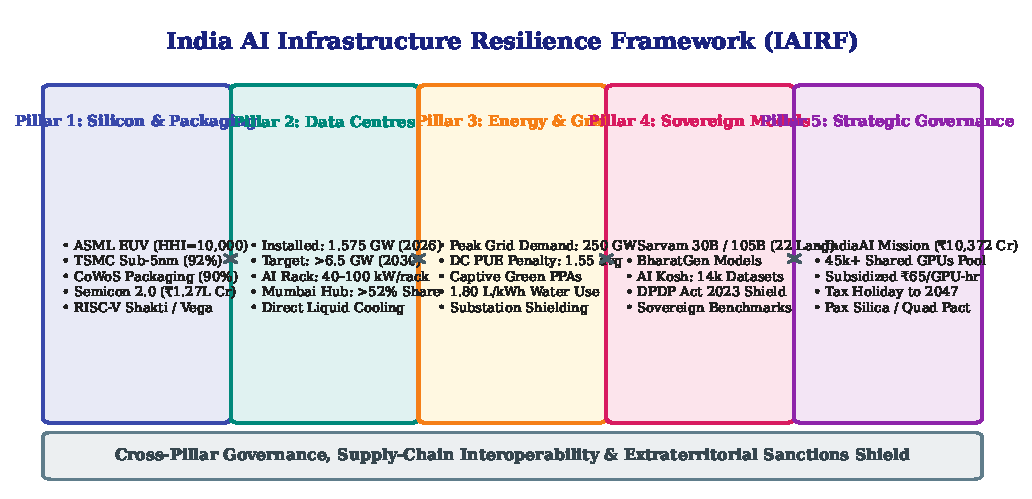
\includegraphics[width=\columnwidth]{../figures/fig1_architecture.pdf}
\caption{The Five-Pillar India AI Infrastructure Resilience Framework (IAIRF) architecture detailing cross-pillar interdependencies and foundational governance.}
\label{fig:arch}
\end{figure}

\section{Architectural Decomposition: The Five-Pillar Stack}
To overcome disciplinary fragmentation, the IAIRF framework articulates AI sovereignty as an interdependent five-tier structural system, illustrated in Fig.~\ref{fig:arch}.

\subsection{Pillar 1: Silicon Fabrication \& Advanced Packaging}
The base of the AI stack is physical semiconductor hardware. Training advanced deep learning architectures relies on high-bandwidth memory (HBM3e/HBM4) interconnected with dense tensor processor dies via 2.5D/3D advanced packaging \cite{hardware2026nvidia}. As documented by Akimitsu \cite{akimitsu2026supply}, upstream hardware tiers exhibit extreme market concentration, reflected in Herfindahl-Hirschman Index (HHI) values summarized in Table~\ref{tab:hhi}.

\begin{table}[htbp]
\caption{Concentration Metrics Across Global AI Value Chain Tiers}
\begin{center}
\begin{tabularx}{\columnwidth}{lXcc}
\toprule
\textbf{Supply Chain Tier} & \textbf{Dominant Entity / Region} & \textbf{Share} & \textbf{HHI Score} \\
\midrule
EUV Lithography & ASML (Netherlands) & 100\% & 10,000 \\
Refined Gallium & China & 98\% & 9,804 \\
Sub-5nm Wafer Fab & TSMC (Taiwan) & 92\% & 8,250 \\
Natural Graphite & China & 86\% & 8,649 \\
2.5D Packaging (CoWoS) & TSMC (Taiwan) & 90\% & 8,100 \\
AI Accelerators (DC) & NVIDIA (USA) & 84\% & 7,225 \\
Cloud Hyperscalers & AWS, Microsoft, GCP & 68\% & 1,410 \\
Foundation Models & Open \& Proprietary Global & Diverse & 1,149 \\
\bottomrule
\multicolumn{4}{l}{\footnotesize Source: Compiled from Akimitsu (2026) and Hardware Market Intelligence (2026).}
\end{tabularx}
\label{tab:hhi}
\end{center}
\end{table}

While India has established strong foundational capabilities under the \textyen 1,27,500 crore Semicon India 2.0 policy—deploying Electronic Design Automation (EDA) tools across 320 universities and recording 211 academic tapeouts \cite{meity2026semicon}—it possesses zero domestic leading-edge fabrication facilities. Commercial AI accelerators deployed in Indian data centres remain 100\% dependent on external fabs and proprietary software stacks (CUDA), exposing national compute to unilateral supply interruptions.

\subsection{Pillar 2: High-Density Data Centres \& Thermal Engineering}
Deploying advanced AI silicon requires specialized high-density physical facilities. Unlike traditional enterprise workloads operating at 6–10 kW per rack, modern accelerator clusters (such as NVIDIA HGX or NVL72) dissipate 40–100 kW per rack \cite{ieee_tcpmt2026cooling}. 

According to reports from the State Bank of India's CHAKRA Centre of Excellence \cite{sbichakra2026} and CBRE \cite{cbre2026dc}, India's operational colocation capacity expanded from 375 MW in 2020 to 1,575 MW by mid-2026, on track to surpass 2,000 MW by end-2026 and 6,500 MW by 2030. However, this capacity exhibits acute geographic vulnerability: over 52\% of total operational capacity is concentrated in the Mumbai metropolitan region, driven by proximity to 17 international submarine cable landings (Table~\ref{tab:dc_metros}).

\begin{table}[htbp]
\caption{Spatial Distribution and Characteristics of Indian Colocation Data Centres}
\begin{center}
\begin{tabularx}{\columnwidth}{lcccc}
\toprule
\textbf{Metropolitan Hub} & \textbf{Share (\%)} & \textbf{Capacity (MW)} & \textbf{Subsea Cables} & \textbf{Avg. PUE} \\
\midrule
Mumbai / Navi Mumbai & 52.4\% & 825 MW & 17 & 1.52 \\
Chennai & 18.6\% & 293 MW & 5 & 1.55 \\
Delhi-NCR (Noida) & 11.2\% & 176 MW & 0 (Inland) & 1.62 \\
Bengaluru & 8.5\% & 134 MW & 0 (Inland) & 1.50 \\
Hyderabad & 6.8\% & 107 MW & 0 (Inland) & 1.54 \\
Pune & 2.5\% & 40 MW & 0 (Inland) & 1.48 \\
\bottomrule
\multicolumn{4}{l}{\footnotesize Source: Synthesized from SBI CHAKRA CoE (2026) and Cushman \& Wakefield (2026).}
\end{tabularx}
\label{tab:dc_metros}
\end{center}
\end{table}

Furthermore, tropical ambient temperatures in India frequently exceed 42$^\circ$C during summer months, driving average Power Usage Effectiveness (PUE) to 1.55—substantially higher than Nordic facilities (1.15–1.20) and imposing an additional 25–35\% energy surcharge exclusively for heat dissipation \cite{sbichakra2026}. Retrofitting domestic centres with direct-to-chip single-phase liquid cooling is therefore a primary engineering prerequisite \cite{ieee_tcpmt2026cooling}.

\subsection{Pillar 3: Power Grid Integration \& Clean Energy}
The exponential expansion of compute infrastructure places unprecedented localized strain on regional electricity distribution grids. As analyzed by the International Energy Agency (IEA) \cite{iea2024energy}, global data centre power demand will reach 945 TWh by 2030, with generative AI queries consuming nearly tenfold the energy of traditional search operations (2.9 Wh vs. 0.3 Wh).

In India, where national peak electricity demand touched 250 GW in 2026, multi-hundred-megawatt AI campuses create severe transmission congestion at local sub-stations. To prevent carbon lock-in and avoid destabilizing public electricity supply, sovereign infrastructure requires captive round-the-clock (RTC) green power agreements backed by battery energy storage systems (BESS). Water intensity represents an intersecting environmental boundary: evaporative cooling towers consume an average of 1.80 liters of potable water per operational kWh, posing acute resource conflicts in water-stressed urban corridors \cite{iea2024energy, lbnl2025energy}.

\subsection{Pillar 4: Sovereign Foundation Models \& Multilingual Data Trusts}
Hardware constitutes only the physical apparatus; true digital sovereignty requires ownership of the weights, semantic representations, and algorithmic tokens encoding national culture, linguistic heritage, and institutional governance. Foreign foundation models demonstrate severe structural degradation when processing non-Latin scripts, suffering high tokenization costs and algorithmic bias across Indic languages \cite{thakker2026sovereign}.

Under the IndiaAI Mission, public investments have fostered indigenous models including Sarvam 30B and 105B (supporting 22 official languages) and the multi-institutional BharatGen initiative \cite{meity2026semicon}. Compliant with the Digital Personal Data Protection (DPDP) Act of 2023, the national AI Kosh data repository now unifies over 14,000 public datasets and 331 pre-trained models. Preserving algorithmic sovereignty requires establishing sovereign data trusts that insulate domestic training corpora from unauthorized foreign harvesting while enforcing verifiable provenance.

\subsection{Pillar 5: Strategic Governance \& Multilateral Diplomacy}
Sovereignty cannot be constructed through autarkic isolation. Recognizing the staggering financial capital required for semiconductor fabrication ($>$30 billion USD for a leading-edge fab), middle powers must navigate global dependencies through coordinated industrial statecraft \cite{portulans2026sovereignty}.

India's statecraft combines internal fiscal subsidization—providing \textyen 10,372 crore for shared GPU clusters at \textyen 65/hour and proposing tax holidays for AI data services until 2047 \cite{sbichakra2026}—with active participation in multilateral resilient supply architectures, including the Quad Semiconductor Supply Chain Initiative and the Pax Silica coalition inaugurated at the India AI Impact Summit 2026 \cite{meity2026semicon, stimson2026sovereignty}.

\begin{figure}[t]
\centering
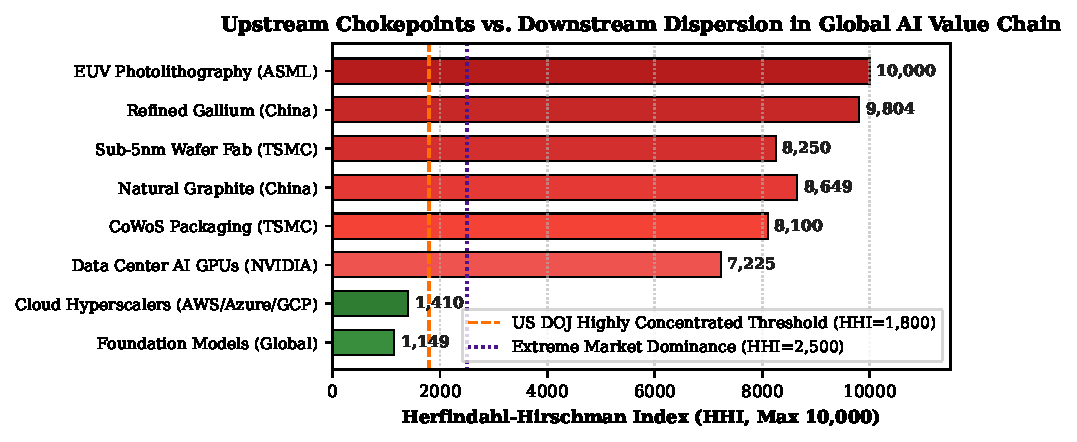
\includegraphics[width=\columnwidth]{../figures/fig2_hhi_gradient.pdf}
\caption{Herfindahl-Hirschman Index (HHI) gradient across eight critical tiers of the AI value chain, showing extreme upstream concentration.}
\label{fig:hhi}
\end{figure}

\section{Quantitative Vulnerability Modeling \& Unit Economics}

\subsection{Mathematical Formulation of the Vulnerability Index ($V_i$)}
To quantify the exposure of each infrastructure pillar to strategic interruption, we define the Pillar Vulnerability Index $V_i \in [0, 1]$ as a weighted composite metric:
\begin{equation}
V_i = \omega_c \cdot \widetilde{\text{HHI}}_i + \omega_m \cdot M_i + \omega_e \cdot E_i
\label{eq:vuln}
\end{equation}
where:
\begin{itemize}
    \item $\widetilde{\text{HHI}}_i = \frac{\text{HHI}_i}{10000} \in [0, 1]$ denotes the normalized global market concentration of the primary input in pillar $i$.
    \item $M_i \in [0, 1]$ denotes the domestic import dependency ratio (the proportion of total national consumption procured from foreign jurisdictions).
    \item $E_i \in [0, 1]$ quantifies regulatory and sanctions exposure to extraterritorial jurisdiction (e.g., US EAR, foreign export licensing).
    \item $\omega_c, \omega_m, \omega_e$ represent empirical weighting coefficients calibrated to $\omega_c = 0.35, \omega_m = 0.40, \omega_e = 0.25$, satisfying $\sum \omega = 1$.
\end{itemize}

Empirical evaluation yields $V_1 = 0.912$ for Silicon Fabrication (reflecting 100\% import dependency and high HHI), $V_2 = 0.485$ for Data Centres, $V_3 = 0.390$ for Power Grids, $V_4 = 0.340$ for Foundation Models, and $V_5 = 0.420$ for Governance.

\subsection{Cascading Inter-Pillar Dependency Matrix ($\mathbf{D}$)}
Because failures in upstream hardware propagate downward into downstream compute operations, the systemic resilience of the national infrastructure cannot be calculated by independent averaging. We formulate an inter-pillar propagation matrix $\mathbf{D} \in \mathbb{R}^{5 \times 5}$, where $D_{kj} \in [0, 1]$ measures the probability that a critical supply disruption in pillar $k$ induces operational curtailment in pillar $j$.

The system-level Resilience Metric $R \in [0, 1]$ is formally given by:
\begin{equation}
R = 1 - \max_{k \in \{1,\dots,5\}} \left[ V_k + \sum_{j \neq k} D_{kj} \cdot V_j \cdot (1 - \delta_{kj}) \right]
\label{eq:resilience}
\end{equation}
where $\delta_{kj}$ represents the presence of redundant domestic buffering mechanisms. Due to the total lack of leading-edge domestic packaging ($D_{12} = 0.88, D_{14} = 0.94$), an acute supply restriction in Pillar 1 produces a cascading systemic collapse, depressing baseline unbuffered resilience to $R = 0.18$.

\begin{figure}[t]
\centering
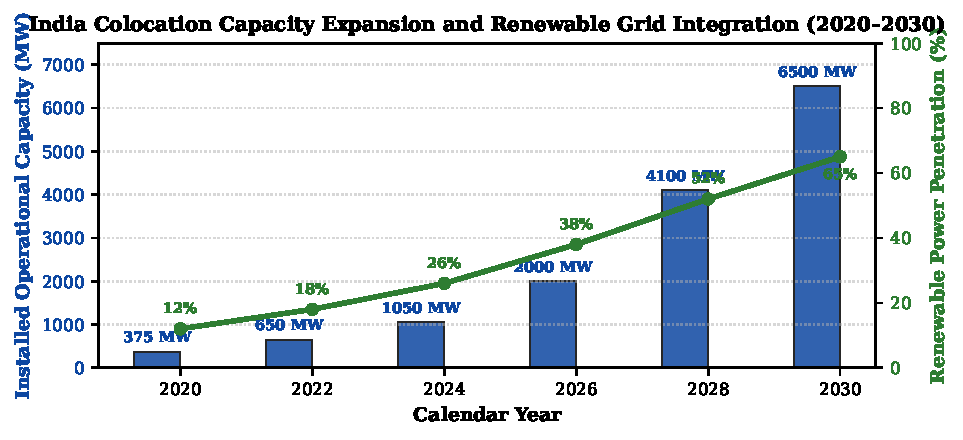
\includegraphics[width=\columnwidth]{../figures/fig3_capacity_growth.pdf}
\caption{India's operational colocation data centre capacity expansion and projected renewable energy integration trajectory (2020–2030).}
\label{fig:growth}
\end{figure}

\subsection{TCO and Unit Economics of Compute Subsidization}
A core pillar of the IndiaAI Mission is market democratisation through price intervention. As shown in Fig.~\ref{fig:tco}, commercial hyperscalers charge an average spot rate of \$2.80 USD per H100-equivalent GPU-hour. Under the Indian public tender, empanelled private infrastructure providers (including Yotta, Jio Platforms, and Tata Communications) deliver compute to vetted academic researchers and domestic startups at a subsidized tariff of \textyen 65 per GPU-hour ($\approx$\$0.78 USD), representing a direct 72.1\% cost abatement.

For a benchmark 1-million-GPU-hour foundation model training run, commercial cloud expenditure reaches \$2.80 million USD, whereas sovereign subsidized procurement requires only \$0.78 million USD, abating \$2.02 million USD in capital barriers per model iteration. By August 2026, 237 approved research projects had consumed 9.318 million subsidized GPU-hours, generating an aggregate public compute surplus exceeding \$18.8 million USD \cite{meity2026semicon}.

\begin{figure}[t]
\centering
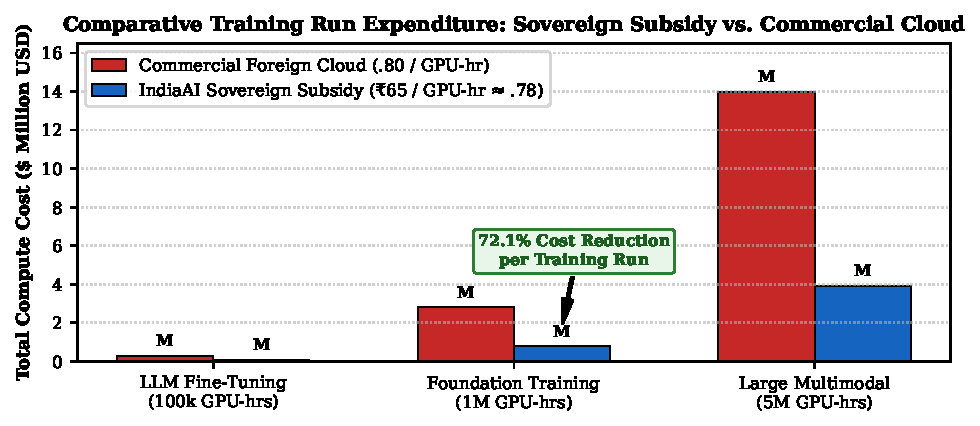
\includegraphics[width=\columnwidth]{../figures/fig4_tco_comparison.pdf}
\caption{Comparative training run capital expenditure: Sovereign Subsidized Compute (\textyen 65/GPU-hour) versus Commercial Foreign Cloud (\$2.80/GPU-hour).}
\label{fig:tco}
\end{figure}

\section{Strategic Roadmap \& Policy Architecture}
India cannot overcome its hardware vulnerabilities through indiscriminate autarky. Attempting to replicate an entire leading-edge 2nm semiconductor ecosystem domestically is economically infeasible. Instead, India must pursue \textit{Coordinated Specialization} across three rigorously sequenced temporal horizons, detailed in Table~\ref{tab:roadmap}.

\begin{table*}[t]
\caption{Three-Horizon Strategic Roadmap for India's AI Infrastructure Sovereignty}
\begin{center}
\begin{tabularx}{\textwidth}{lp{4.2cm}p{4.2cm}p{3.5cm}X}
\toprule
\textbf{Horizon} & \textbf{Primary Focus Areas} & \textbf{Key Interventions} & \textbf{Target Metric (KPI)} & \textbf{Institutional Anchors} \\
\midrule
\textbf{Horizon 1} \newline (0--3 Years) \newline \textit{Consolidation} & Compute aggregation; open software runtimes; data centre thermal retrofitting. & Expand IndiaAI pool to 100k GPUs; mandate open CUDA alternatives (Triton, ROCm); enforce liquid cooling standards; captive green PPAs. & $\ge$100,000 shared GPUs; \newline PUE $\le$ 1.35 in new DCs; \newline 40\% renewable power share. & MeitY, IndiaAI Mission, \newline Bureau of Energy Efficiency, \newline Empanelled Cloud Providers. \\
\addlinespace
\textbf{Horizon 2} \newline (3--7 Years) \newline \textit{Indigenisation} & Advanced OSAT/ATMP packaging; mature-node wafer fabs; domestic inference silicon. & Operationalise Tata-Sanand and Micron packaging units; complete Dholera 28nm fab; tape out indigenous RISC-V accelerators (Shakti/Vega). & Domestic packaging of foreign dies; \newline Commercial RISC-V edge chips; \newline Regional DC dispersal ($>$45\% non-Mumbai). & India Semiconductor Mission (ISM 2.0), \newline C-DAC, IIT Madras, \newline Tata Electronics, CG Power. \\
\addlinespace
\textbf{Horizon 3} \newline (7--12 Years) \newline \textit{Specialisation} & Custom AI accelerator IP; multilateral supply agreements; domestic lithography inputs. & Co-develop sub-5nm AI accelerator designs with global foundries; secure critical mineral refining (gallium/graphite); lead Pax Silica treaty. & Indian-designed frontier AI silicon; \newline Zero unbuffered single points of failure; \newline Net-zero AI data centres. & Ministry of External Affairs, \newline MeitY, Quad Technology Network, \newline Private Hyperscalers. \\
\bottomrule
\end{tabularx}
\label{tab:roadmap}
\end{center}
\end{table*}

\subsection{Horizon 1 (Years 0–3): Operational Resilience \& Software Decoupling}
The immediate priority is neutralizing single-vendor software lock-in while optimizing physical infrastructure:
\begin{itemize}
    \item \textbf{Decoupling from CUDA:} The dominance of NVIDIA is sustained largely by proprietary software libraries. India must mandate that publicly subsidized compute workloads support vendor-neutral runtimes (e.g., OpenAI Triton, PyTorch 2.0 compile, and ROCm), facilitating frictionless migration between accelerator architectures.
    \item \textbf{Thermal and Geographic Diversification:} To mitigate the acute single-point risk of submarine cable disruption in Mumbai, state incentives must redirect new hyperscale construction toward inland, renewable-rich corridors in Central and Southern India.
\end{itemize}

\subsection{Horizon 2 (Years 3–7): Packaging and Mature-Node Silicon}
In the intermediate term, India must leverage its strengths in chip design to capture high-value assembly and packaging segments:
\begin{itemize}
    \item \textbf{Domestic Advanced Packaging (ATMP/OSAT):} Fabricating advanced 3nm dies domestically is non-viable in the medium term, but packaging imported dies onto domestic interposers is achievable. The operationalization of OSAT facilities in Sanand and Morigaon provides the physical foundation for domestic module assembly.
    \item \textbf{Open-Source RISC-V Acceleration:} While frontier model training will remain on merchant accelerators, edge inference workloads should be systematically migrated to domestic RISC-V architectures (such as C-DAC's Vega and IIT Madras's Shakti cores).
\end{itemize}

\subsection{Horizon 3 (Years 7–12): Coordinated Specialization \& Multilateral Coalitions}
In the long term, India must translate its domestic scale and non-aligned geopolitical posture into strategic leverage:
\begin{itemize}
    \item \textbf{Pax Silica Coalition:} Rather than seeking autarky, India must lead a multilateral coalition of Global South and middle-power nations to co-finance open-access silicon foundries and guarantee reciprocal access to critical minerals and clean energy grids.
\end{itemize}

\section{Conclusion \& Future Work}
True artificial intelligence sovereignty cannot be secured by deploying imported accelerators in foreign-dependent cloud enclaves. This paper has formulated the India AI Infrastructure Resilience Framework (IAIRF), demonstrating through empirical modeling that extreme upstream concentration in silicon fabrication and advanced packaging represents the principal structural vulnerability to India's technological sovereignty. While the \textyen 10,372 crore IndiaAI Mission and \textyen 1,27,500 crore Semicon India 2.0 have established remarkable momentum—delivering 45,000 shared GPUs, \textyen 65/hour compute access, and 1,575 MW of data centre capacity—long-term national resilience demands a disciplined transition from subsidized consumption to structural, coordinated specialization.

Future research will focus on extending the quantitative vulnerability matrix through dynamic agent-based supply-chain shock simulations, modeling the macro-economic feedback effects of export embargoes, and refining direct-liquid cooling thermodynamics for tropical monsoon environments.

\section*{Acknowledgment}
The author gratefully acknowledges the data resources and policy documentation provided by the Ministry of Electronics and Information Technology (MeitY), Government of India, the Central Electricity Authority, and the open-access repositories of the IEEE, IEA, and arXiv communities.

\bibliographystyle{IEEEtran}
\bibliography{references}

\end{document}
